\section{Domänenmodellierung}

\begin{definition}{Domänenmodell}
Ein Domänenmodell ist ein vereinfachtes UML-Klassendiagramm zur Darstellung der Fachdomäne:
\begin{itemize}
    \item Konzepte als Klassen
    \item Eigenschaften als Attribute (ohne Typangabe)
    \item Beziehungen als Assoziationen mit Multiplizitäten
\end{itemize}
\includegraphics[width=\linewidth]{images/domänenmodell.png}
\end{definition}

\begin{KR}{Domänenmodell Erstellung}
\textbf{1. Konzepte identifizieren}
\begin{itemize}
    \item \textbf{Kategorien prüfen:}
    \begin{itemize}
        \item Physische Objekte (Produkte, Geräte)
        \item Kataloge und Listen
        \item Container (Warenkorb, Lager)
        \item Externe Systeme
        \item Rollen von Personen
        \item Artefakte (Dokumente, Verträge)
        \item Zahlungsinstrumente
    \end{itemize}
    \item \textbf{Wichtig:} Keine Softwareklassen modellieren!
\end{itemize}

\textbf{2. Attribute definieren}
\begin{itemize}
    \item Nur wichtige/zentrale Attribute
    \item \textbf{Typische Kategorien:}
    \begin{itemize}
        \item Transaktionsdaten
        \item Teil-Ganzes Beziehungen
        \item Beschreibungen
    \end{itemize}
    \item \textbf{Wichtig:}
    \begin{itemize}
        \item Beziehungen als Assoziationen, nicht als Attribute
        \item Keine technischen IDs
        \item Keine abgeleiteten Werte
    \end{itemize}
\end{itemize}

\textbf{3. Beziehungen modellieren}
\begin{itemize}
    \item Assoziationen zwischen Konzepten identifizieren
    \item Multiplizitäten festlegen
    \item Art der Beziehung bestimmen
    \item Richtung der Assoziation falls nötig
\end{itemize}
\end{KR}

\subsection{Analysemuster}

\begin{formula}{Analysemuster im Überblick}
Bewährte Strukturen für wiederkehrende Modellierungssituationen:
\begin{itemize}
    \item \textbf{Beschreibungsklassen:} Trennung von Typ und Instanz
    \item \textbf{Generalisierung:} "ist-ein" Beziehungen
    \item \textbf{Komposition:} Starke Teil-Ganzes Beziehung
    \item \textbf{Zustände:} Eigene Zustandshierarchie
    \item \textbf{Rollen:} Verschiedene Funktionen eines Konzepts
    \item \textbf{Assoziationsklasse:} Attribute einer Beziehung
\end{itemize}
\end{formula}

\begin{concept}{Beschreibungsklassen}
Trennt die Beschreibung eines Typs von seinen konkreten Instanzen:
\begin{itemize}
    \item Verwendung bei mehreren gleichartigen Objekten
    \item Gemeinsame unveränderliche Eigenschaften
    \item Vermeidung von Redundanz
\end{itemize}
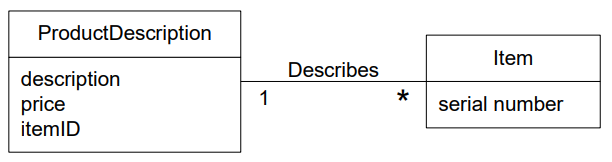
\includegraphics[width=0.9\linewidth]{images/beschreibungsklasse_better.png}
\end{concept}

\begin{concept}{Generalisierung/Spezialisierung}
\textbf{Regeln:}
\begin{itemize}
    \item 100% Regel: Jede Instanz der Spezialisierung ist auch Instanz der Generalisierung
    \item 'IS-A' Beziehung
    \item Gemeinsame Attribute/Assoziationen in Basisklasse
    \item Spezifische Eigenschaften in Unterklassen
\end{itemize}
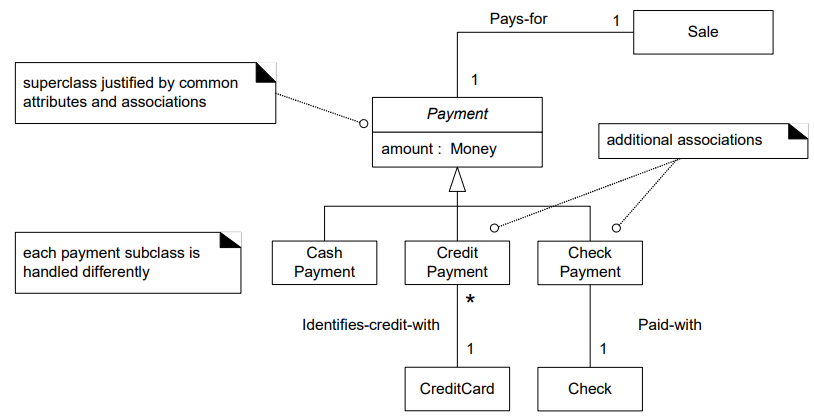
\includegraphics[width=0.9\linewidth]{images/generalisierung_extended.png}
\end{concept}

\begin{concept}{Zustände}
\begin{itemize}
    \item Modellierung als eigene Konzepthierarchie
    \item Vermeidung problematischer Vererbung
    \item Erweiterbarkeit durch neue Zustandsklassen
\end{itemize}
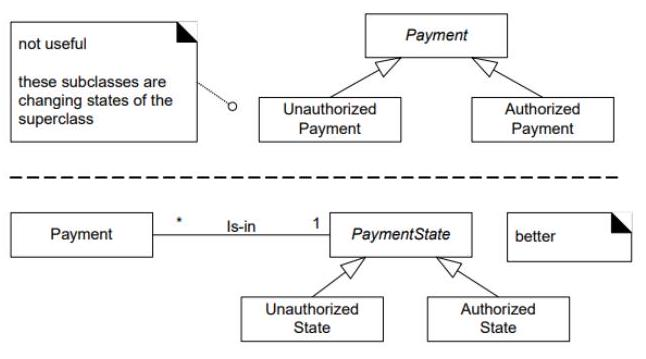
\includegraphics[width=0.9\linewidth]{images/2024_12_29_0d1d7b5551ea1b4b41bdg-07(1)}
\end{concept}

\begin{concept}{Assoziationsklassen}
\textbf{Einsatz wenn:}
\begin{itemize}
    \item Attribute zur Beziehung gehören
    \item Beziehung eigene Identität hat
    \item Mehrere Beziehungen möglich sind
\end{itemize}
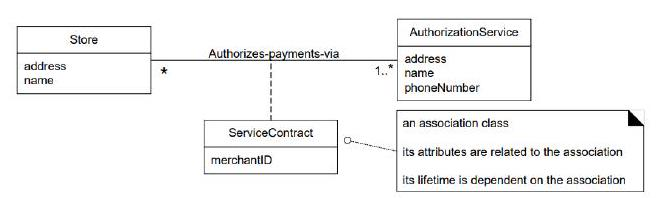
\includegraphics[width=\linewidth]{images/2024_12_29_0d1d7b5551ea1b4b41bdg-07}
\end{concept}

%todo: Add examples for each pattern type

\begin{definition}{Optionale Elemente im Domänenmodell}
\begin{itemize}
    \item Optional: Aggregationen/Kompositionen
\end{itemize}
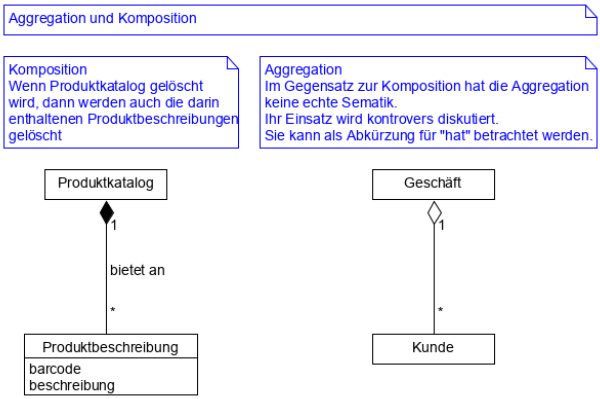
\includegraphics[width=\linewidth]{images/aggregation_komposition.png}
\begin{itemize}
    \item Optional: Generalisierung/Spezialisierung
\end{itemize}
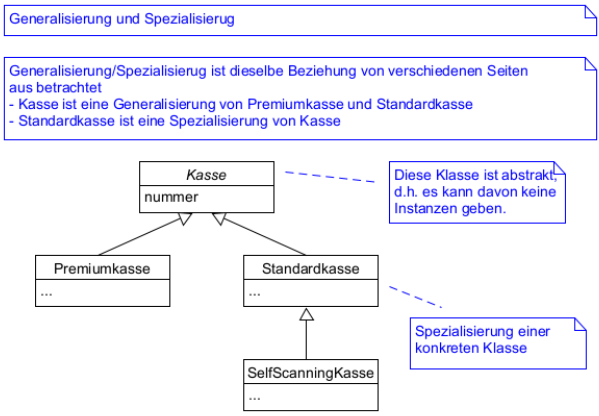
\includegraphics[width=\linewidth]{images/gener_spez.png}
\end{definition}

%todo: Add complete example of a domain model